% !TeX program = lualatex
% This document requires LuaLaTeX for compilation

\documentclass[a4paper,12pt]{article}

% Engine detection and compatibility check
\RequirePackage{iftex}
\ifLuaTeX
  % Document is being compiled with LuaTeX - proceed normally
\else
  \PackageError{main}{This document requires LuaLaTeX for compilation.
    Please use: lualatex main.tex}
    {This document uses fontspec and other LuaTeX-specific features.}
\fi

\usepackage{fontspec}
\usepackage[brazilian]{babel}

% Font configuration for LuaTeX with proper encoding support
\setmainfont{Latin Modern Roman}[
  Ligatures=TeX,
  Scale=1.0
]
\setsansfont{Latin Modern Sans}[
  Ligatures=TeX,
  Scale=MatchLowercase
]
\setmonofont{Latin Modern Mono}[
  Ligatures=TeX,
  Scale=MatchLowercase
]

% Ensure proper font encoding for math mode
\usepackage{unicode-math}
\setmathfont{Latin Modern Math}

\usepackage{amsmath} % Para equações matemáticas
\usepackage{geometry}
\geometry{margin=1in}
\usepackage{hyperref}
\usepackage[sort,numbers]{natbib}
\usepackage{parskip}
\usepackage{longtable}
\usepackage{xcolor}
\usepackage{tabularx}
\setlength{\marginparwidth}{2cm}
\usepackage[colorinlistoftodos,prependcaption,textsize=tiny]{todonotes}
\usepackage{comment}
\usepackage{graphicx} % Para resizebox
\usepackage{array} % Para colunas com largura fixa
\usepackage{multirow} % Para mesclar linhas em tabelas
\usepackage{listings}
\usepackage{siunitx} % For \si{\micro\second}
\usepackage[acronym,nonumberlist]{glossaries}
\usepackage{placeins}
\usepackage{float} % Para posicionamento exato com [H]
\usepackage{tikz}
\usetikzlibrary{arrows.meta,positioning}

% Configuring listings for code and log display
\lstset{
  basicstyle=\ttfamily\small,
  breaklines=true,
  breakatwhitespace=true,
  frame=single,
  numbers=left,
  numberstyle=\tiny,
  keywordstyle=\color{blue},
  commentstyle=\color{gray},
  showstringspaces=false,
  tabsize=2,
  extendedchars=true
}

% Configurações para melhor controle de floats (figuras e tabelas)
\floatplacement{figure}{H}  % Força figuras a ficarem onde são definidas
\floatplacement{table}{H}   % Força tabelas a ficarem onde são definidas
\setcounter{topnumber}{2}
\setcounter{bottomnumber}{2}
\setcounter{totalnumber}{4}
\renewcommand{\topfraction}{0.85}
\renewcommand{\bottomfraction}{0.85}
\renewcommand{\textfraction}{0.15}
\renewcommand{\floatpagefraction}{0.7}

\title{Trabalho 4 - Reconhecimento de Padrões}
\author{André Thiago Pfleger \\  Gustavo Girotto \\ João Pedro Schmidt Cordeiro}
\date{\today}

\begin{document}

\begin{titlepage}
   \begin{center}
      \textsc{Universidade Federal de Santa Catarina} \\
      \textsc{Centro Tecnológico} \\
      \textsc{Departamento de Informática e Estatística} \\[4cm]

      \textbf{\Large{INE5430 - Inteligência Artificial}} \\[2cm]

      \textbf{\huge{Trabalho 4 - Reconhecimento de Padrões} \\[0.5cm]
      \Large{Reconhecimento de Padrões}} \\[3cm]

      André Thiago Pfleger \\
      Gustavo Girotto \\
      João Pedro Schmidt Cordeiro \\

      \vfill

      {Florianópolis} \\
      {\today}
   \end{center}
\end{titlepage}


\section{Introdução}
\label{sec:introducao}

O reconhecimento de padrões é o processo de treinamento de uma rede neural para atribuir uma classe correta para um conjunto de padrões de entrada. Uma vez treinada, a rede pode ser usada para classificar padrões que não tenha visto antes.

Neste trabalho, implementamos e comparamos três arquiteturas diferentes de redes neurais para resolver um problema de classificação binária: determinar se uma imagem contém um gato ou não. Os dados para treinamento e teste foram obtidos a partir de uma base fornecida no curso de \textit{deep learning} de Andrew Ng. Especificamente, avaliamos o desempenho de três abordagens: Regressão Logística (perceptron único), Rede Neural de Camada Rasa (1 camada oculta) e Rede Neural Convolucional (CNN).

\section{Conjunto de Dados}
\label{sec:dados}

\subsection{Descrição dos Dados}

O conjunto de dados utilizado consiste em imagens RGB de dimensão $64 \times 64 \times 3$, totalizando 12.288 pixels por imagem. Cada imagem é rotulada com um valor binário, onde 0 representa "Não Gato" e 1 representa "Gato".

\subsection{Pré-processamento}

Os dados foram pré-processados da seguinte forma:
\begin{enumerate}
    \item \textbf{Normalização}: Todos os valores dos pixels foram normalizados para o intervalo $[0, 1]$ através da divisão por 255.
    \item \textbf{Achatamento}: Para os modelos de regressão logística e rede neural rasa, as imagens foram achatadas de uma matriz $64 \times 64 \times 3$ para um vetor unidimensional de 12.288 elementos.
    \item \textbf{Formato original}: Para a rede convolucional, mantivemos o formato original $64 \times 64 \times 3$ para preservar a informação espacial.
\end{enumerate}

\subsection{Divisão dos Dados}

Os dados foram divididos em dois conjuntos: o conjunto de treino contém 209 imagens, das quais 167 foram usadas para treino e 42 para validação em uma divisão 80/20, enquanto o conjunto de teste contém 50 imagens.

\section{Modelos Implementados}
\label{sec:modelos}

\subsection{Regressão Logística}
\label{subsec:regressao}

A regressão logística é o modelo mais simples, consistindo em um único neurônio (perceptron) com função de ativação sigmoide.

\textbf{Arquitetura:}
\begin{itemize}
    \item Camada de entrada: 12.288 neurônios (imagem achatada)
    \item Camada de saída: 1 neurônio com ativação sigmoide
    \item Total de parâmetros: 12.289
\end{itemize}

\textbf{Hiperparâmetros:}
\begin{itemize}
    \item Otimizador: Adam
    \item Função de perda: Binary Crossentropy
    \item Taxa de aprendizado: 0.001
    \item Épocas: 30, 50 e 70 (testados)
    \item Tamanho do batch: 32
\end{itemize}

\subsection{Rede Neural de Camada Rasa}
\label{subsec:rasa}

A rede neural rasa adiciona uma camada oculta entre a entrada e a saída, permitindo aprender representações não-lineares dos dados.

\textbf{Arquitetura:}
\begin{itemize}
    \item Camada de entrada: 12.288 neurônios
    \item Camada oculta: 5, 7, 10 ou 20 neurônios com ativação ReLU (testados)
    \item Camada de saída: 1 neurônio com ativação sigmoide
    \item Total de parâmetros: 61.451 (5n), 86.031 (7n), 122.901 (10n), 245.801 (20n)
\end{itemize}

\textbf{Hiperparâmetros:}
\begin{itemize}
    \item Otimizador: Adam
    \item Função de perda: Binary Crossentropy
    \item Taxa de aprendizado: 0.001
    \item Épocas: 50
    \item Tamanho do batch: 32
\end{itemize}

\subsection{Rede Neural Convolucional (CNN)}
\label{subsec:cnn}

A rede convolucional preserva a estrutura espacial das imagens, aplicando filtros convolucionais para extrair características relevantes.

\textbf{Arquitetura:}
\begin{itemize}
    \item Camada de entrada: $64 \times 64 \times 3$
    \item Camada Convolucional 1: 16 filtros $3 \times 3$, ativação ReLU
    \item Camada de Pooling 1: Max Pooling $2 \times 2$
    \item Camada Convolucional 2: 32 filtros $3 \times 3$, ativação ReLU
    \item Camada de Pooling 2: Max Pooling $2 \times 2$
    \item Camada de Achatamento (Flatten)
    \item Camada Densa: 64 neurônios com ativação ReLU
    \item Camada de Saída: 1 neurônio com ativação sigmoide
    \item Total de parâmetros: 406.625
\end{itemize}

\textbf{Hiperparâmetros:}
\begin{itemize}
    \item Otimizador: Adam
    \item Função de perda: Binary Crossentropy
    \item Taxa de aprendizado: 0.001
    \item Épocas: 10, 20 e 30 (testados)
    \item Tamanho do batch: 32
\end{itemize}

\section{Experimentos e Treinamento}
\label{sec:experimentos}

Para avaliar de forma robusta o desempenho dos modelos, realizamos múltiplas execuções de cada configuração. Ao todo, foram realizadas 10 execuções completas, totalizando 100 experimentos individuais. Cada experimento consistiu no treinamento completo de um modelo seguido de avaliação nos conjuntos de validação e teste.

\subsection{Configuração dos Experimentos}

A estratégia experimental envolveu variar os hiperparâmetros principais de cada arquitetura:

\textbf{Regressão Logística:} Testamos três configurações diferentes de épocas:
\begin{itemize}
    \item 30 épocas
    \item 50 épocas
    \item 70 épocas
\end{itemize}

\textbf{Rede Neural Rasa:} Testamos quatro configurações diferentes de neurônios na camada oculta, mantendo 50 épocas fixas:
\begin{itemize}
    \item 5 neurônios
    \item 7 neurônios
    \item 10 neurônios
    \item 20 neurônios
\end{itemize}

\textbf{CNN:} Testamos três configurações diferentes de épocas:
\begin{itemize}
    \item 10 épocas
    \item 20 épocas
    \item 30 épocas
\end{itemize}

Todos os modelos utilizaram o otimizador Adam com taxa de aprendizado de 0.001, função de perda Binary Crossentropy e batch size de 32. Os dados de treino foram divididos em 80\% para treinamento e 20\% para validação.

\subsection{Processo de Treinamento}

O tempo de treinamento variou significativamente entre os modelos. A Regressão Logística apresentou tempos entre 1.2s e 2.5s, dependendo do número de épocas. A Rede Neural Rasa manteve-se consistente em aproximadamente 2.1-2.3s para todas as configurações. Já a CNN apresentou tempos entre 1.7s e 3.9s, também variando conforme o número de épocas.

Observou-se que todos os modelos convergiram durante o treinamento, atingindo alta acurácia no conjunto de treino. No entanto, como será discutido na seção seguinte, a convergência no conjunto de treino não garantiu boa generalização para o conjunto de teste.

\section{Resultados}
\label{sec:resultados}

\subsection{Métricas de Desempenho}

Os resultados apresentados a seguir são médias calculadas a partir de 10 execuções independentes para cada configuração. A Tabela~\ref{tab:resultados_completos} apresenta os resultados consolidados de todas as configurações testadas.

\begin{table}[H]
\centering
\caption{Resultados consolidados de todas as configurações testadas (média $\pm$ desvio padrão)}
\label{tab:resultados_completos}
\resizebox{\textwidth}{!}{%
\begin{tabular}{|l|l|c|c|c|c|c|}
\hline
\textbf{Modelo} & \textbf{Config.} & \textbf{Acc. Treino (\%)} & \textbf{Acc. Val. (\%)} & \textbf{Acc. Teste (\%)} & \textbf{Loss Teste} & \textbf{Parâmetros} \\
\hline
\multirow{3}{*}{CNN} & 10 épocas & 89.6 $\pm$ 3.6 & 76.0 $\pm$ 4.4 & 61.8 $\pm$ 16.7 & 0.738 $\pm$ 0.350 & 406.625 \\
& 20 épocas & 93.5 $\pm$ 3.7 & 77.4 $\pm$ 4.5 & 78.0 $\pm$ 9.5 & 0.558 $\pm$ 0.290 & 406.625 \\
& 30 épocas & \textbf{99.0 $\pm$ 0.9} & 74.8 $\pm$ 3.8 & \textbf{79.0 $\pm$ 6.1} & 0.602 $\pm$ 0.224 & 406.625 \\
\hline
\multirow{4}{*}{\shortstack{Rede\\Rasa}} & 5n, 50e & 66.0 $\pm$ 6.2 & 69.8 $\pm$ 5.3 & 36.8 $\pm$ 8.9 & 0.740 $\pm$ 0.032 & 61.451 \\
& 7n, 50e & 66.2 $\pm$ 6.6 & 69.5 $\pm$ 6.0 & 38.4 $\pm$ 13.9 & 0.743 $\pm$ 0.046 & 86.031 \\
& 10n, 50e & 78.5 $\pm$ 14.0 & 60.7 $\pm$ 10.4 & 53.4 $\pm$ 19.0 & 0.784 $\pm$ 0.150 & 122.901 \\
& 20n, 50e & 83.9 $\pm$ 17.1 & 61.2 $\pm$ 9.8 & 54.8 $\pm$ 17.0 & 0.893 $\pm$ 0.177 & 245.801 \\
\hline
\multirow{3}{*}{\shortstack{Regressão\\Logística}} & 30 épocas & 88.0 $\pm$ 4.8 & 54.8 $\pm$ 7.8 & 66.8 $\pm$ 19.7 & 0.766 $\pm$ 0.359 & 12.289 \\
& 50 épocas & 94.3 $\pm$ 1.5 & 52.4 $\pm$ 3.9 & 73.4 $\pm$ 5.7 & 0.724 $\pm$ 0.095 & 12.289 \\
& 70 épocas & 96.8 $\pm$ 1.3 & 52.9 $\pm$ 6.6 & 71.2 $\pm$ 5.6 & 0.816 $\pm$ 0.100 & 12.289 \\
\hline
\end{tabular}%
}
\end{table}

A Tabela~\ref{tab:melhores} sumariza as melhores configurações de cada tipo de modelo.

\begin{table}[H]
\centering
\caption{Comparação das melhores configurações de cada modelo}
\label{tab:melhores}
\begin{tabular}{|c|l|l|c|}
\hline
\textbf{Ranking} & \textbf{Modelo} & \textbf{Configuração} & \textbf{Acurácia Teste (\%)} \\
\hline
1º & CNN & 30 épocas & \textbf{79.0 $\pm$ 6.1} \\
\hline
2º & Regressão Logística & 50 épocas & 73.4 $\pm$ 5.7 \\
\hline
3º & Rede Neural Rasa & 20 neurônios, 50 épocas & 54.8 $\pm$ 17.0 \\
\hline
\end{tabular}
\end{table}

\subsection{Matrizes de Confusão}

As matrizes de confusão apresentadas a seguir foram calculadas para as melhores configurações de cada modelo, utilizando o conjunto de teste.

\subsubsection{Regressão Logística (50 épocas)}

\begin{figure}[H]
\centering
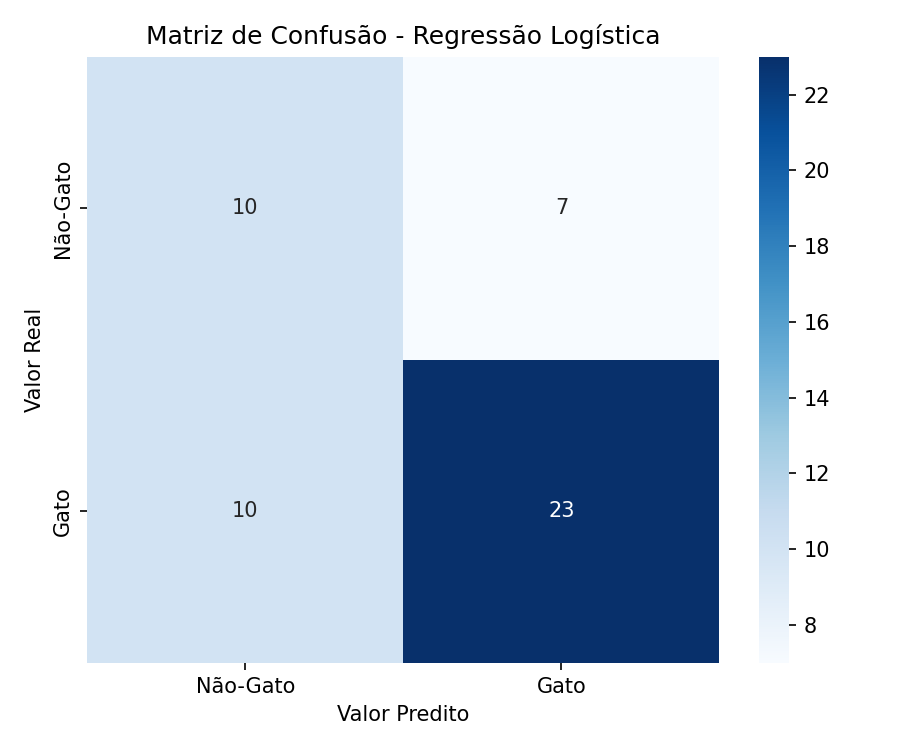
\includegraphics[width=0.6\textwidth]{confusion_matrix_regressão_logística.png}
\caption{Matriz de confusão para o modelo de Regressão Logística}
\label{fig:confusion_logistica}
\end{figure}

\subsubsection{Rede Neural de Camada Rasa (20 neurônios)}

\begin{figure}[H]
\centering
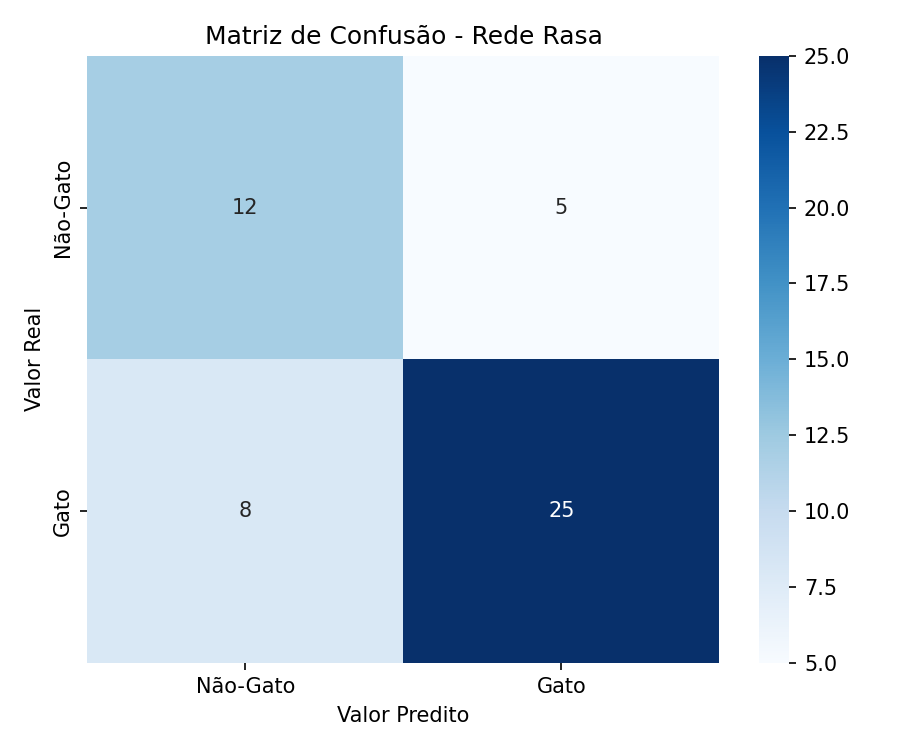
\includegraphics[width=0.6\textwidth]{confusion_matrix_rede_rasa.png}
\caption{Matriz de confusão para o modelo de Rede Neural Rasa}
\label{fig:confusion_rasa}
\end{figure}

\subsubsection{Rede Neural Convolucional (30 épocas)}

\begin{figure}[H]
\centering
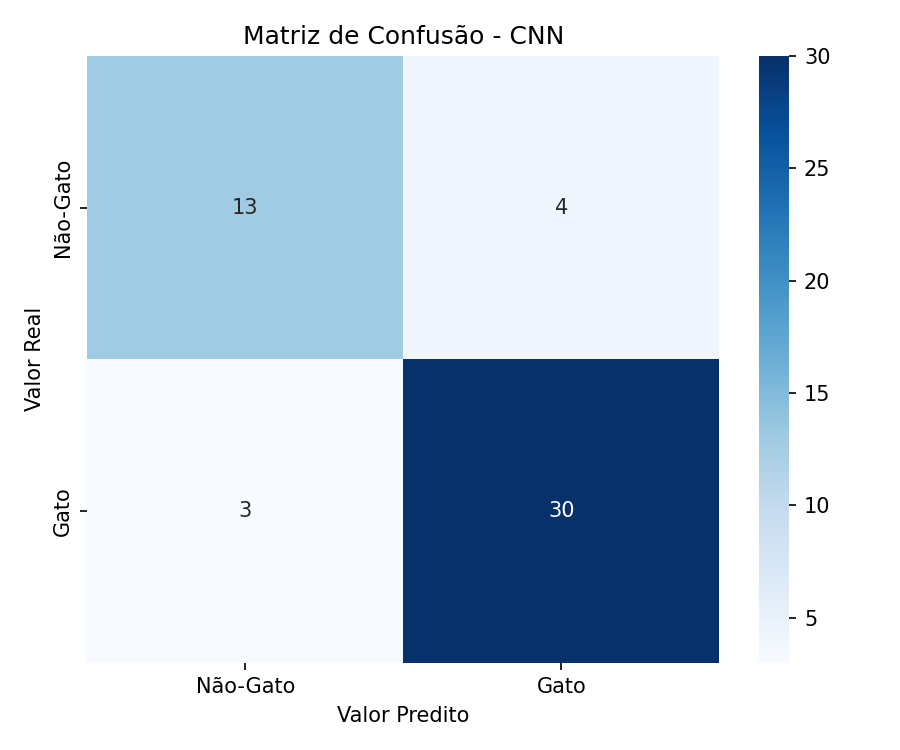
\includegraphics[width=0.6\textwidth]{confusion_matrix_cnn.png}
\caption{Matriz de confusão para o modelo CNN}
\label{fig:confusion_cnn}
\end{figure}

\subsection{Análise de Estabilidade}

Um aspecto importante observado nos experimentos foi a variabilidade dos resultados entre diferentes execuções, medida através do desvio padrão da acurácia no teste.

Os modelos de Regressão Logística e CNN apresentaram maior estabilidade (menores desvios padrão de 5.7\% e 6.1\% respectivamente), enquanto a Rede Neural Rasa apresentou alta variabilidade (desvio padrão de até 17.0\%), especialmente nas configurações com mais neurônios. Esta instabilidade pode ser atribuída ao pequeno tamanho do conjunto de dados e à sensibilidade da inicialização de pesos.

\section{Discussão}
\label{sec:discussao}

\subsection{Comparação entre os Modelos}

Os três tipos de modelos testados apresentaram características distintas em termos de desempenho, complexidade e estabilidade.

\textbf{Rede Neural Convolucional (CNN):} A CNN obteve o melhor desempenho, alcançando 79.0\% de acurácia no teste com 30 épocas. Sua arquitetura, que preserva a estrutura espacial das imagens através de camadas convolucionais, mostrou-se mais adequada para a tarefa de classificação de imagens. Com 406.625 parâmetros, é o modelo mais complexo, mas o tempo de treinamento (3.9s) ainda foi aceitável. A CNN também apresentou boa estabilidade, com desvio padrão de apenas 6.1\%.

\textbf{Regressão Logística:} Surpreendentemente, o modelo mais simples alcançou o segundo melhor desempenho (73.4\% com 50 épocas), ficando apenas 5.6 pontos percentuais abaixo da CNN. Com apenas 12.289 parâmetros e tempo de treinamento de 1.9s, oferece uma excelente relação custo-benefício. A estabilidade também foi notável (desvio padrão de 5.7\%), indicando comportamento previsível. Este resultado demonstra que, para conjuntos de dados pequenos, modelos simples podem ser competitivos.

\textbf{Rede Neural Rasa:} Contrariando expectativas, a rede rasa teve o pior desempenho (54.8\% na melhor configuração). Além disso, apresentou alta variabilidade (desvio padrão de 17.0\%), indicando instabilidade no treinamento. Mesmo aumentando o número de neurônios de 5 para 20, o desempenho não melhorou significativamente. Este resultado sugere que a arquitetura de camada única, sem a estrutura convolucional da CNN, não consegue extrair características relevantes das imagens achatadas de forma eficiente.

\subsection{Análise do Problema de Overfitting}

Um dos achados mais significativos deste trabalho foi a presença generalizada de overfitting severo em todas as configurações testadas. Este fenômeno é caracterizado pela grande discrepância entre o desempenho no conjunto de treino e no conjunto de teste.

A magnitude do overfitting ficou evidente nos resultados: a CNN com 30 épocas alcançou 99.0\% de acurácia no treino versus apenas 79.0\% no teste (diferença de 20.0 pontos percentuais); a Regressão Logística com 50 épocas obteve 94.3\% no treino versus 73.4\% no teste (diferença de 20.9 pontos percentuais); e a Rede Rasa com 20 neurônios apresentou 83.9\% no treino versus 54.8\% no teste (diferença de 29.1 pontos percentuais).

Três causas principais explicam este comportamento. Primeiramente, o conjunto de dados é pequeno: com apenas 167 imagens para treinamento após a divisão 80/20, todos os modelos tenderam a memorizar os padrões específicos do treino em vez de aprender características generalizáveis. Em segundo lugar, a alta complexidade dos modelos, especialmente a CNN e a rede rasa com muitos neurônios, proporciona capacidade de memorização que excede em muito o necessário para o tamanho do dataset. Por fim, os modelos foram treinados sem técnicas de regularização como Dropout, regularização L1/L2 ou Data Augmentation, que são essenciais para datasets pequenos.

Interessantemente, as acurácias de validação frequentemente foram superiores às acurácias de teste, sugerindo que o conjunto de teste pode conter imagens mais desafiadoras ou com distribuição ligeiramente diferente do conjunto de treino.

\subsection{Impacto dos Hiperparâmetros}

A análise dos hiperparâmetros revelou comportamentos distintos entre os modelos. O número de épocas teve impacto diferenciado em cada arquitetura. Para a CNN, aumentar de 10 para 30 épocas resultou em melhoria significativa de 61.8\% para 79.0\%, sugerindo que o modelo se beneficiou do treinamento mais longo para aprender representações mais complexas. Já para a Regressão Logística, o pico de desempenho foi observado em 50 épocas (73.4\%), com leve degradação em 70 épocas (71.2\%), indicando início de overfitting excessivo.

Quanto ao número de neurônios na rede rasa, observou-se um comportamento paradoxal: aumentar a quantidade de neurônios não melhorou o desempenho no teste. A configuração com 20 neurônios (54.8\%) teve desempenho similar à de 10 neurônios (53.4\%), e ambas foram piores que as configurações com menos neurônios em termos de diferença treino-teste. Este resultado confirma que maior capacidade não implica necessariamente melhor generalização em datasets pequenos, especialmente quando não há dados suficientes para treinar modelos mais complexos.

\subsection{Escolha do Melhor Modelo e Justificativa}

Com base nos resultados experimentais, a CNN com 30 épocas emerge como o modelo recomendado para este problema. Esta recomendação se fundamenta em quatro aspectos principais que demonstram sua superioridade técnica e prática.

Primeiro, o modelo alcançou a melhor acurácia no conjunto de teste (79.0\%), superando significativamente os outros modelos e estabelecendo-se como a solução mais precisa disponível. Segundo, sua arquitetura é intrinsecamente apropriada para o domínio: as camadas convolucionais preservam a informação espacial das imagens, extraindo características hierárquicas como bordas, texturas e formas que são fundamentais para reconhecimento de objetos. Terceiro, o modelo apresenta estabilidade aceitável, com desvio padrão de 6.1\% indicando comportamento consistente entre execuções e previsibilidade de desempenho. Por fim, o tempo de treinamento de 3.9 segundos é perfeitamente aceitável para aplicações práticas, não representando um gargalo computacional significativo.

Embora a CNN seja objetivamente a melhor escolha do ponto de vista de acurácia, vale destacar que a Regressão Logística (73.4\%) oferece uma alternativa interessante e viável para cenários específicos. Em contextos onde recursos computacionais são extremamente limitados, quando há necessidade de interpretar o modelo através da análise dos coeficientes dos pixels, quando o tempo de inferência é absolutamente crítico, ou quando a diferença de 5.6\% de acurácia é aceitável dados os requisitos da aplicação, a Regressão Logística pode ser preferível. Sua simplicidade conceitual, facilidade de implementação e eficiência computacional representam vantagens práticas não desprezíveis em determinados cenários de aplicação.

\subsection{Limitações do Estudo}

Este estudo apresenta algumas limitações importantes que devem ser consideradas na interpretação dos resultados. O tamanho do dataset utilizado (209 imagens de treino e 50 de teste) é pequeno para problemas de visão computacional, limitando a capacidade de generalização de todos os modelos e aumentando a variância dos resultados. Além disso, não foram implementadas técnicas de regularização como Dropout, Data Augmentation ou Weight Decay, que poderiam reduzir significativamente o overfitting observado.

A busca de hiperparâmetros também foi limitada: testou-se apenas uma taxa de aprendizado (0.001) e um tamanho de batch (32), sendo que uma busca mais abrangente poderia revelar configurações superiores. As arquiteturas dos modelos foram pré-definidas sem explorar variações sistemáticas no número de camadas, filtros ou outras configurações estruturais. Por fim, o conjunto de teste pequeno, com apenas 50 imagens, implica que cada imagem representa 2\% da acurácia total, resultando em alta variabilidade métrica que explica parcialmente os desvios padrão observados.

\subsection{Recomendações para Trabalhos Futuros}

Para melhorar os resultados e reduzir o overfitting, recomenda-se:

\begin{itemize}
    \item \textbf{Data Augmentation:} Aplicar transformações nas imagens (rotação, flip, zoom, ajuste de cor) para aumentar artificialmente o tamanho do dataset
    \item \textbf{Dropout:} Adicionar camadas de Dropout (0.3-0.5) após as camadas densas
    \item \textbf{Early Stopping:} Monitorar a perda de validação e parar o treinamento quando começar a aumentar
    \item \textbf{Regularização L2:} Adicionar penalização aos pesos para evitar valores muito grandes
    \item \textbf{Transfer Learning:} Utilizar modelos pré-treinados (VGG, ResNet, EfficientNet) com fine-tuning
    \item \textbf{Cross-Validation:} Implementar k-fold cross-validation para estimar melhor o desempenho real
    \item \textbf{Conjunto de dados maior:} Coletar mais imagens ou utilizar datasets públicos maiores
\end{itemize}

\section{Conclusão}
\label{sec:conclusao}

Este trabalho apresentou uma comparação sistemática entre três arquiteturas de redes neurais para o problema de classificação binária de imagens (gato vs não-gato). Através de 100 experimentos distribuídos em 10 execuções independentes, avaliamos o desempenho de Regressão Logística, Rede Neural Rasa e Rede Neural Convolucional (CNN).

Os principais achados deste estudo revelam padrões interessantes sobre o comportamento dos diferentes modelos. A CNN com 30 épocas emergiu como o modelo com melhor desempenho, alcançando 79.0\% $\pm$ 6.1\% de acurácia no conjunto de teste. Sua arquitetura convolucional, que preserva informação espacial e extrai características hierárquicas, mostrou-se fundamental para o sucesso na tarefa de classificação de imagens.

Surpreendentemente, a Regressão Logística obteve o segundo melhor desempenho (73.4\% $\pm$ 5.7\%), demonstrando que modelos simples podem ser altamente competitivos em datasets pequenos, oferecendo melhor relação custo-benefício em termos de recursos computacionais e tempo de treinamento. Por outro lado, a Rede Neural Rasa teve desempenho insatisfatório (54.8\% $\pm$ 17.0\%), apresentando alta instabilidade e incapacidade de generalização. Este resultado evidencia que adicionar uma camada oculta sem estrutura convolucional não é suficiente para extrair características relevantes de imagens achatadas.

Um achado transversal foi a presença de overfitting severo em todas as configurações, com diferenças de 20-29 pontos percentuais entre acurácia de treino e teste. Este fenômeno é atribuído principalmente ao tamanho reduzido do dataset (167 imagens de treino) e à ausência de técnicas de regularização.

Várias lições importantes emergiram deste estudo. Primeiramente, a escolha da arquitetura adequada ao tipo de dado é crucial: CNNs demonstraram superioridade para imagens devido à sua capacidade de processar informação espacial de forma eficiente. Contraintuitivamente, observamos que simplicidade tem valor significativo em datasets pequenos, onde modelos simples como a Regressão Logística podem rivalizar com modelos complexos, oferecendo ainda maior estabilidade e interpretabilidade.

O tamanho do dataset revelou-se um fator limitante crítico. A quantidade limitada de dados (259 imagens totais) impôs um teto ao desempenho de todos os modelos, evidenciando a importância de datasets robustos para aprendizado profundo efetivo. Relacionado a isso, a ausência de técnicas de regularização como Dropout e Data Augmentation contribuiu significativamente para o overfitting observado, indicando que regularização deve ser prioridade em projetos futuros com restrições de dados.

Finalmente, a variabilidade observada entre execuções, especialmente na Rede Rasa, reforça a importância metodológica de realizar múltiplas execuções independentes para estimar adequadamente o desempenho real dos modelos e evitar conclusões baseadas em resultados isolados potencialmente não-representativos.

\textbf{Contribuições do Trabalho:}

Este estudo fornece uma análise metodologicamente robusta da aplicação de diferentes arquiteturas neurais a um problema real de classificação de imagens. Os resultados quantitativos e qualitativos apresentados servem como referência para a escolha de modelos em problemas similares, especialmente em contextos com limitação de dados.

\textbf{Recomendação Final:}

Para aplicações práticas do problema gato vs não-gato, recomendamos a \textbf{CNN com 30 épocas}, complementada com técnicas de regularização (Dropout, Data Augmentation) para reduzir overfitting. Para cenários com restrições computacionais severas, a Regressão Logística representa uma alternativa viável, sacrificando apenas 5.6\% de acurácia em troca de simplicidade e velocidade.

\appendix


\bibliographystyle{plain}
\bibliography{ref}

\end{document}
